\chapter{Epistemic marking across the Himalayas}\label{c:Description}
This chapter presents an overview of epistemic marking in the \lfam\ family collected as per Chapter \ref{c:Methodology}.
\section{General Summary}
\subsection{State of description}\label{ss:Description:StateOfDescription}
The level of coverage in the description of languages across the \lfam\ subfamilies varies greatly, ranging from subfamilies with over a hundred published grammars, to a number with no published comprehensive grammars, or even no published description at all. In order to compare the state of description across the family and illustrate the disparities, data on language numbers (also presented in Table \ref{t:Methods:SubfamilyLanguageCount}) as well as on published literature on each language has been collected from Glottolog \cite{glottolog}. Specifically, the number of unique\footnote{This excluded both exact repetitions in the database where two sources have had the same publication under slightly different names (e.g., with or without middle names or initials), and cases where a two grammars of the same language by the same author are listed, usually because of a thesis which has subsequently been turned into a book. This latter case has been excluded as, while there are likely differences between the two publications, they do not represent the greater level of coverage in the literature that would be seen from a second grammar being written out of an entirely separate project.} publications categorised in Glottolog's database as ``Grammar'' has been counted for each subfamily, as well as the languages of these publications. These figures are estimations, given that the boundary between the distinction in the database between ``Grammar'' and ``Grammar Sketch'' is not a clear line\footnote{Glottolog does define the categories as ``~150 pages and beyond'' and ``~50 pages'' \cite[Glossary]{glottolog}, though this is not always reflected in practise.}, and that it is relying on Glottolog's very broad but not necessarily perfect coverage of the literature. Similarly, the figures used for the numbers of languages are, of course, also estimations using Glottolog's categorisation. Finally, the database covers publications on grammars dating back at times to the 19th century, which may not be considered up to contemporary standards in terms of linguistic analysis. As such, these figures can certainly be illustrative in a broad sense, showing the differences in documentation levels in general terms, but cannot be seen as precise figures for any further detailed statistical analysis.

The highest coverage was recorded for Meithei, an internal isolate. Glottolog recorded eight unique grammars for the one language, with the earliest being a description by Arthur John Primrose published in 1888\nocite{Primrose1888}. This is, however, by some measure the highest, with the next highest ratio of languages to grammars seen for the Sinitic subfamily, which has 4.46 grammars for each language\footnote{116 grammars across 26 languages.}. Figure \ref{f:Description:SubfamilyCoverageGraph} shows the ratio of overall grammars per language in each subfamily. Four subfamilies show a ratio of one, meaning there is an equal number of published grammars on the subfamily and languages in the subfamily on Glottolog. This does not mean, however, that every language in the subfamily has been described, as levels of description can vary widely within a given subfamily. While an internal isolate, the example of Meithei is a good explanation of why this is possible, where multiple grammars have been written on the one language. Similarly, there are cases where the authors of grammars might consider two varieties different languages, or at least sufficiently different for a separate grammar, but the varieties are grouped as one langauge on Glottolog. For example, of the two English-language grammars on Tshangla, another internal isolate, \citeA{Grollmann2020} is specifically about the Bjokapakha variety, while \citeA{Andvik2010} covers Tshangla more generally, as external influences prevented him from working with any single given speech community or village. In other cases, for instance with \citesA{Gates2021}{Honkasalo2019} writing about Eastern Geshiza and Mazur Stau, it is not necessarily clear whether or not the two rGyalrongic varieties described ought to be considered different langauges or not, but are in any case considered grammars of the same language in this analysis. In this example, \citeA[1]{Honkasalo2019} refers to the specific subgroup within rGyalrongic as the ``Horpa languages'', while \citeA[12]{Gates2021} uses the same, as well as the more agnostic term ``Horpa lects''.

\begin{figure}
        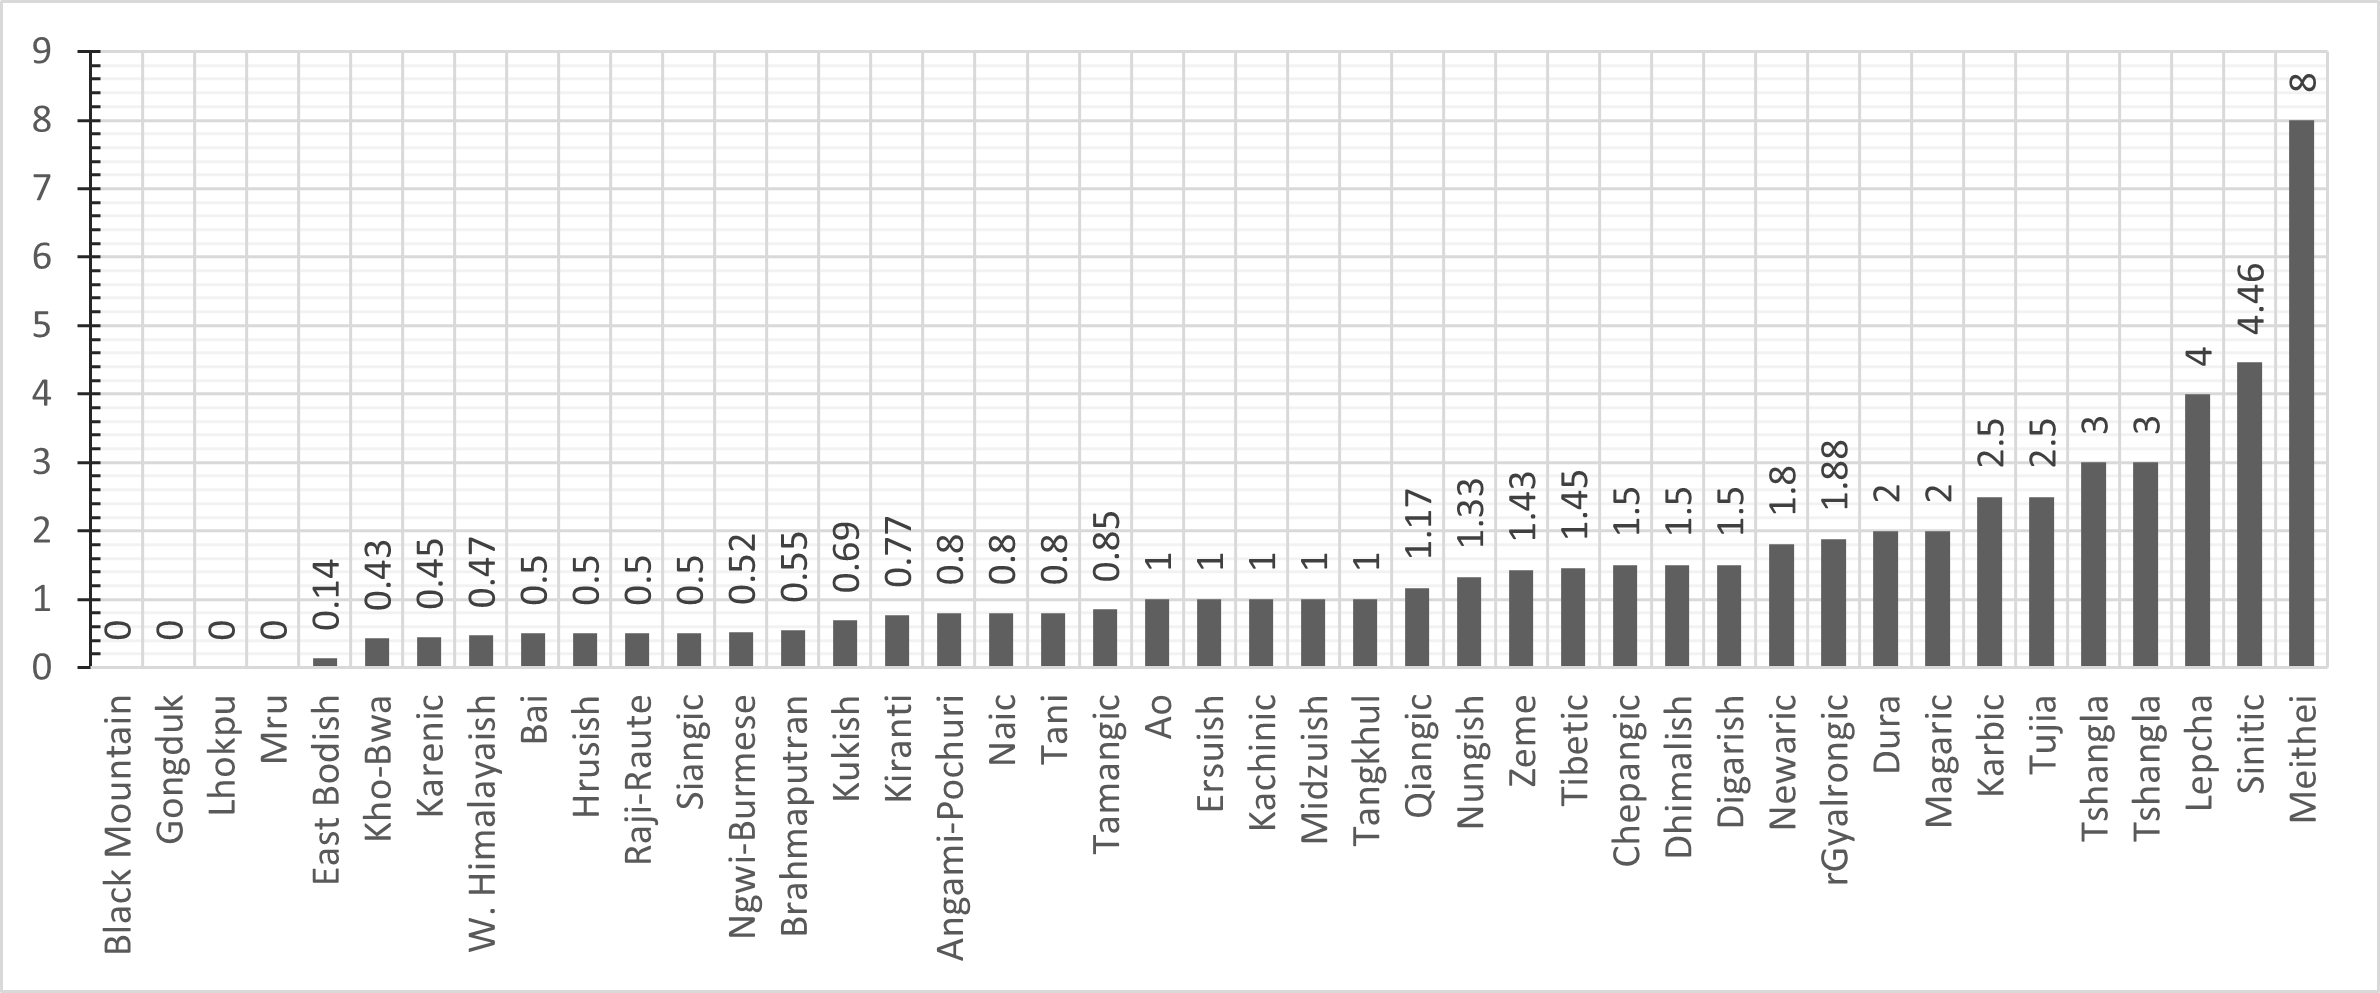
\includegraphics{Subfamily Coverage Graph.png}
        \caption{The ratio of overall grammars per language for each of the subfamilies, sorted from lowest to highest.}\label{f:Description:SubfamilyCoverageGraph}
\end{figure}

A comparison of the metalanguages of the literature in this dataset can also reveal some trends, and more specifically can reveal some gaps in the data that is available to this project, given it was limited to literature written in English with some exceptions in texts written in French or German, e.g. \citeA{Lai2017}. This data is presented in Figure \ref{f:Description:SubfamilyCoverageByLanguage}, showing the metalanguages used as a percentage of the total grammars in the dataset. Unsurprisingly, the families with higher levels of literature in Chinese, namely Bai, Digarish, Ersuish, Kho-Bwa, Mizduish, Ngwi-Burmese, Nungish, Qiangic, rGyalrongic, Sinitic, and Tujia, are all at least in part spoken in China. The Digarish, Kho-Bwa, Midzuish, and Nungish branches are all spoken partly outside of China (or in contested areas), specifically in all three cases around the tri-point between China, Myanmar, and the Indian state of Arunachal Pradesh. In these cases as well, the Chinese literature comprises one or two of a total of three or four publications. The higher level of use of French as a metalanguage in the rGyalronic subfamily (4 out of 15) can be attributed directly to the research and teaching of Guillaume Jacques, as three of the items are doctoral theses over which he was supervisor, and the final is his own grammar of Japhug \cite{Jacques2021}.

\begin{figure}
        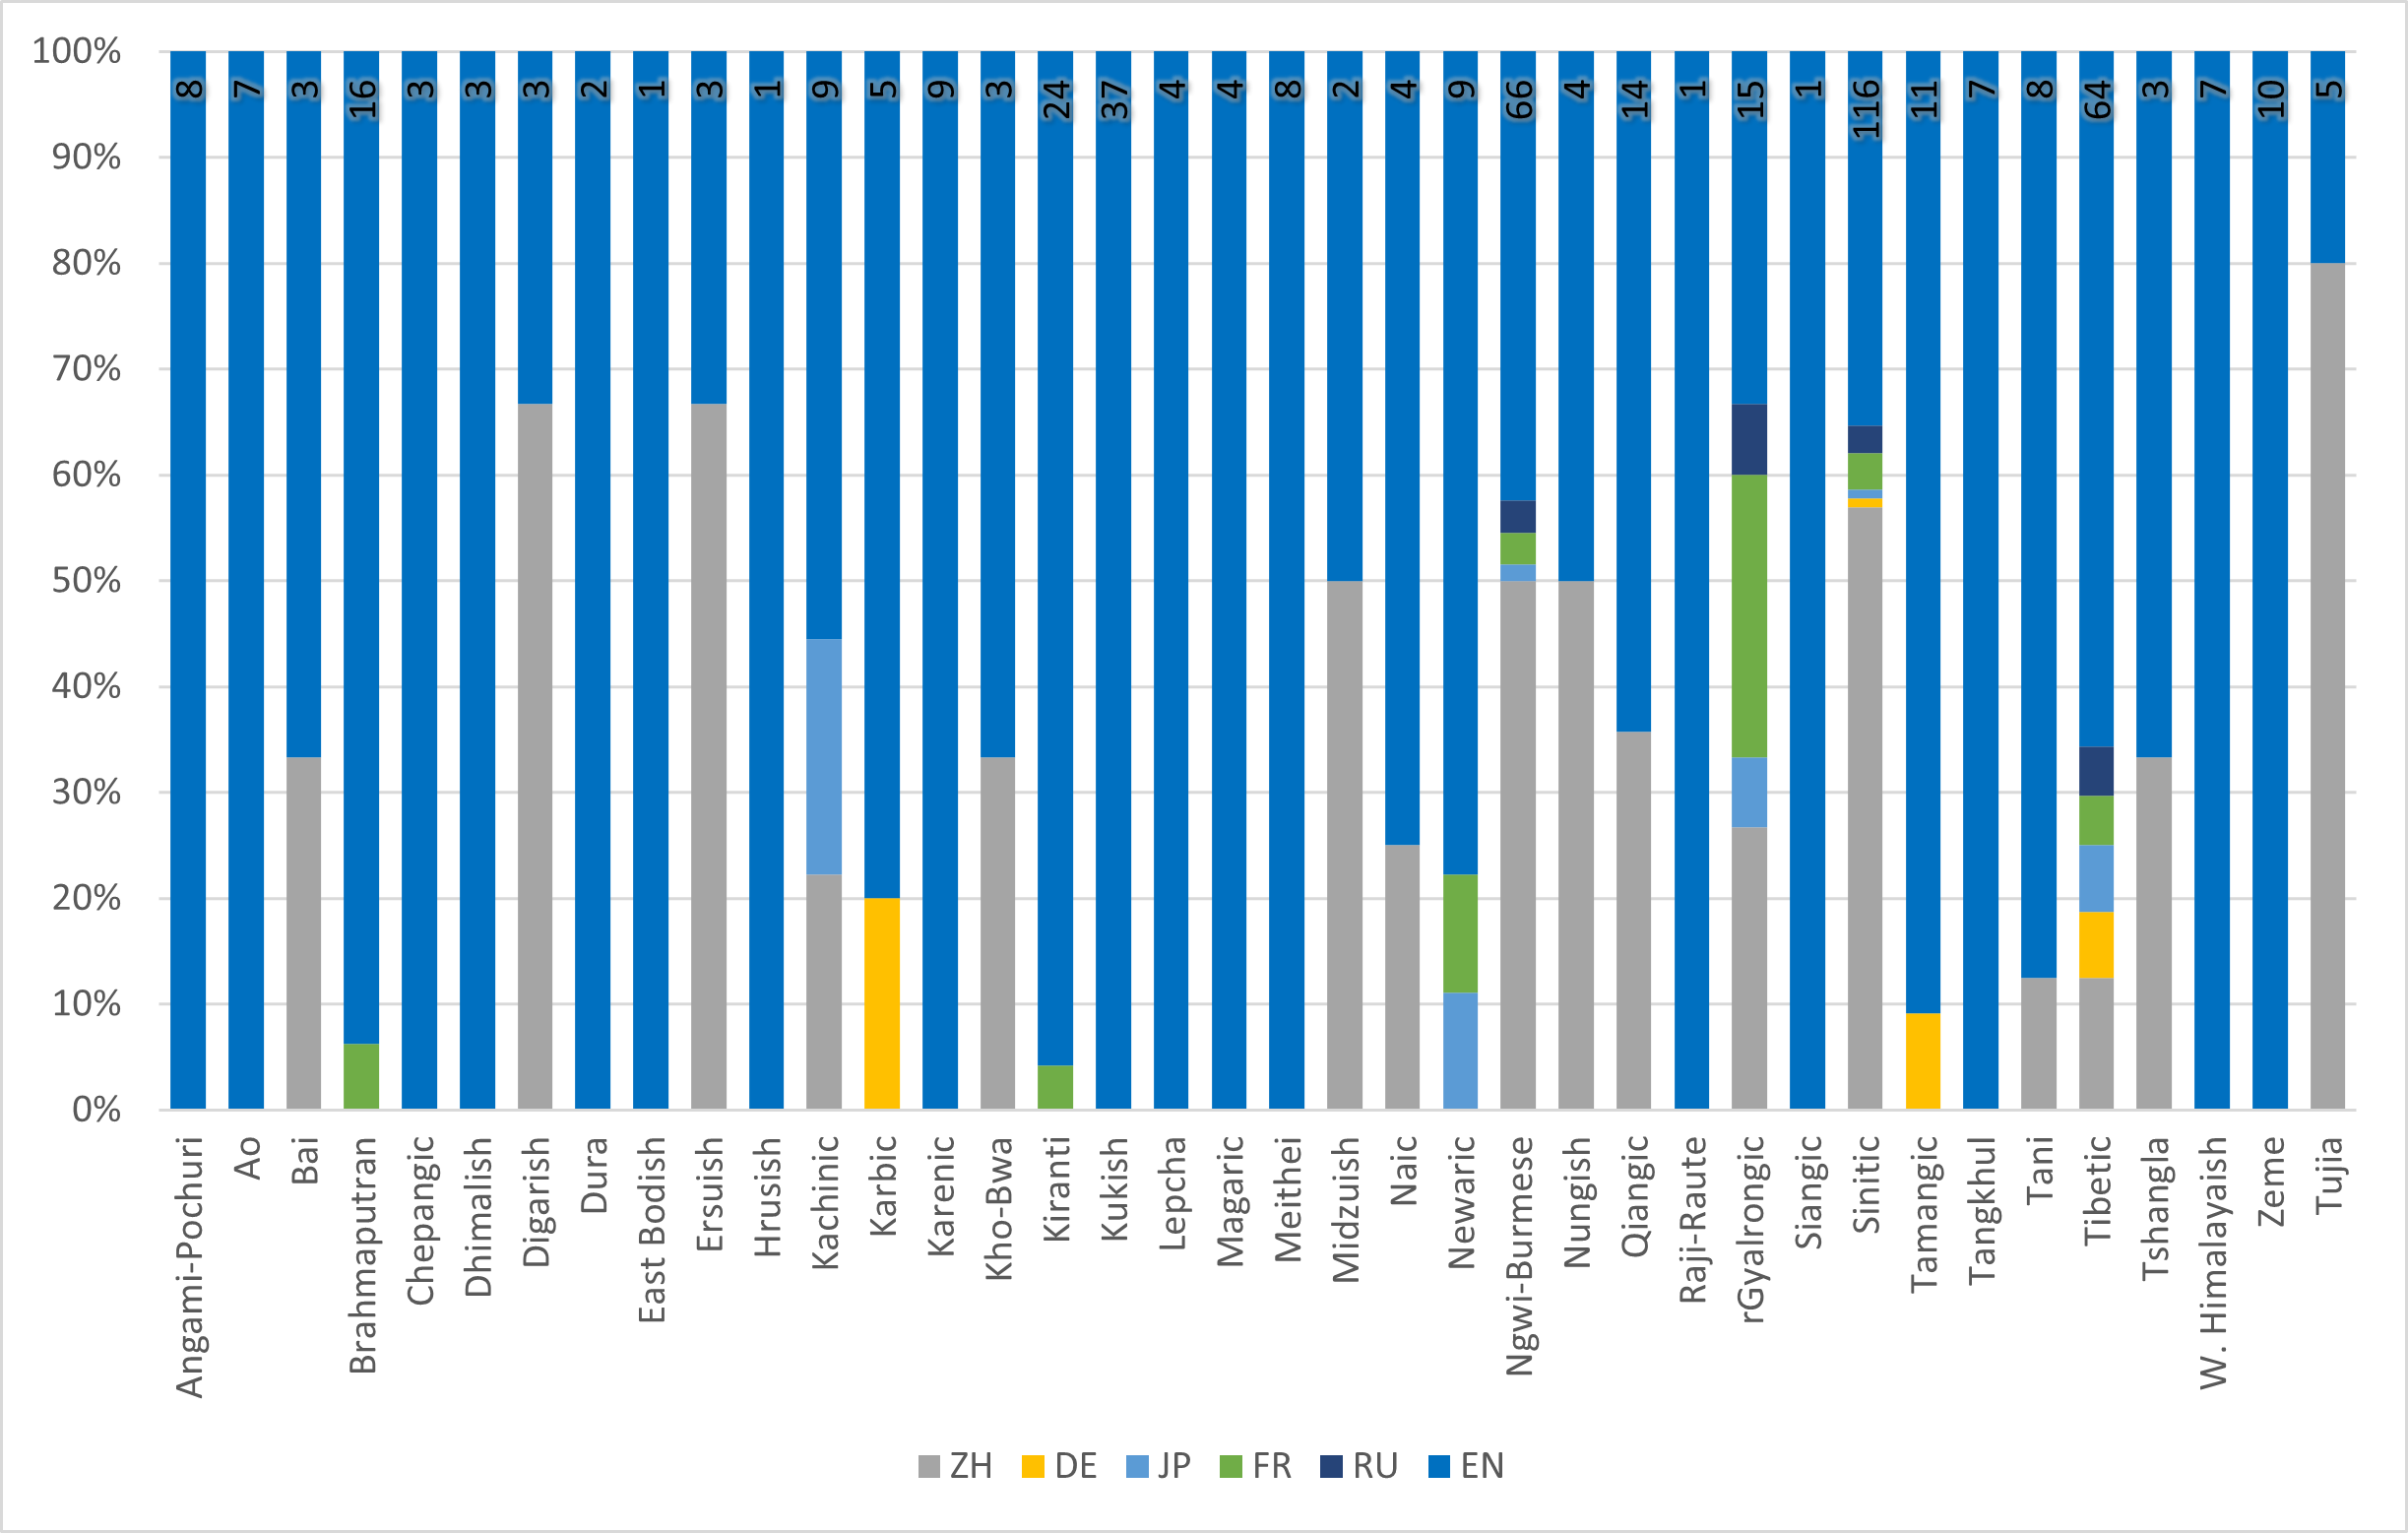
\includegraphics{Subfamily Coverage By Language.png}
        \caption{Distribution of metalanguages as a percentage of the total grammars in each subfamily. The number at the top of each subfamily is the total number of grammars in the dataset per sufamily.}\label{f:Description:SubfamilyCoverageByLanguage}
\end{figure}

Thus far, the literature being referenced in this analysis has broadly been referred to as ``published'' or as a survey of ``publications'', however it is worth noting that this also includes both masters and doctoral theses, which have not technically been published or peer reviewed in the same sense as a book would. While this is not to say that a masters or doctoral thesis is inherently less reliable than a published book, masters theses in particular are inherently shorter and less detailed. It was not feasible to annotate all of the grammars in the dataset for their initial origin in these terms, but assuming a higher number of masters and doctoral students undertaking descriptive projects than degree-holding academics undertaking such projects to the point of a published grammar, it can be assumed that theses comprise a substantial if not majority portion of the dataset\footnote{While this rings true in the current, I suspect that this has not always been the case. Additionally, the rise of theses being readily available online has made them more accessible, and potentially more common in the Glottolog database.}. To compare only the data collected for the larger analysis in this project, discussed in Section \ref{s:Methods:Collection}, about 40\% are masters or doctoral theses, and theses were generally only used where no formally published book was available.

\subsection{Languages with conflicting analyses}\label{ss:Description:Conflicts}
A challenge in taking the analyses presented in the literature at face value is that, in cases where multiple descriptions of a single langauge exist (as discussed in Section \ref{ss:Description:StateOfDescription}), there may be different, conflicting analyses of a particular form or function. This section presents a number of examples of cases where a decision had to be made, and discusses why that decision was made the way it was. 

\paragraph{Sunwar}
In his initial descriptions of mirativity, \citeA{DeLanceyMirativity1997} gives Sunwar (Kiranti: Nepal) as an example of a language showing grammaticalised mirativity. In particular, DeLancey describes the copulas \textit{tshə} and \textit{'baak-} as being distinguished based on the newness of knowledge. DeLancey reports that the use of each copula is conditioned independently of the source of the speaker's knowledge (evidentiality), but is rather conditioned by whether or not the information is known without qualification by the speaker (\textit{tshə}) or is information they have just learned, through any of reportative, inferential, or direct evidence (\textit{'baak-}). Example \ref{e:Description:SunwarMirative} shows this distinction in a minimal pair, with the non-mirative used in situations where the speaker has perhaps lived in Kathmandu and is familiar Tangka and the mirative form used in situations where the speaker perhaps did not know Tangka was in Kathmandu but had just seen him, or had just been told he was there \cite[42]{DeLanceyMirativity1997}.

\begin{exe}
        \ex\label{e:Description:SunwarMirative}
        \begin{xlist}
                \ex 
                \gll Tangka Kathmandu-m tshaa \\
                Tangka Kathmandu-\textsc{loc} \textsc{tsha.3sg} \\
                \glt `Tangka is in Kathmandu.' (non-mirative)

                \ex
                \gll Tangka Kathmandu-m 'baâ-tə \\
                Tangka Kathmandu-\textsc{loc} exist-\textsc{3.sg.past} \\
                \glt `Tangka is in Kathmandu.' (non-mirative)
        \end{xlist}
        \cite[Sunwar][41-42]{DeLanceyMirativity1997}
\end{exe}

\citeA{Borchers2008} disagrees with this analysis, though concedes that she and DeLancey are working with data from different Sunwar-speaking communities, and notes that DeLancey's analysis is working with a smaller corpus than hers. Borchers suggests instead that \textit{'baak-} ``is used to express the general way that things are'', whereas \textit{tshə} ``denotes the concrete and recent state of affairs'' \cite[164]{Borchers2008}. \citeA{Hill2012} is also critical of DeLancey's analysis, though in an overall argument against mirativity as valid cross-linguistic category. That being said, Hill's criticism of the mirative analysis, while referencing \citeA{Borchers2008} for support, relies only on a reanalysis of the meagre data presented in \citeA{DeLanceyMirativity1997} (here in Example \ref{e:Description:SunwarMirative}) and a discussion of edge cases one would not reasonably expect DeLancey to have discussed given the level of detail in the description given in his paper.

The question thus becomes one of which analysis to follow for this typology. That is, in order to enter data from Sunwar into the database, we must make a decision about whose analysis to follow. In this case, given Borchers, at least by her accounts, worked with substantially more data, and spent a much longer time in the field than DeLancey (who worked with a single speaker living in the United States \cite{DeLanceyMirativity1997}). This is, in all reality, a fairly minor decision. It is, in this case, a single point of data in a substantially larger database, and despite Hill's (2012) strong criticism of DeLancey's description, \citeA{Borchers2008} does give a number of possible reasons for the difference in analysis, and does not appear to go to the same length as Hill in actively attempting to refute DeLancey. There also continues to be other languages analysed as marking mirativity in the sample, and as such mirativity as a concept is still considered in this typological analysis.

\paragraph{Lhasa Tibetan}
There is a similar disagreement in the literature over the best way to analyse the evidential system in Lhasa Tibetan, again involving disagreement over the mirative between \citeA{DeLanceyMirativity1997} and \citeA{Hill2012}, though with a greater number of other possible analyses. Epistemic marking in Lhasa Tibetan varies between equative copular clauses, and existential copular and verb clauses. Specifically, there are two epistemic bases in the equative copula system, compared to three in the existential copulas and verbal morphology \cite{DeLancey2017Tibetan}. These forms are given in Table \ref{t:Description:LhasaEpistemics}, adapted from \citeA[11]{Garrett2001} and using his labels for the 2-3 evidential bases. It is the precise labelling of these bases in a theoretical sense that has been debated in the literature.

\begin{table}
        \begin{tabular}{llll}
         & Ego & Direct & Indirect \\
        Equative Copulas & \textit{yin} & \multicolumn{2}{l}{\textit{red}} \\
        Existential Copulas & \textit{yod} & \textit{ḥdug} & \textit{yodred} \\
        Verbal Morphology (past)\footnote{This paradigm is conditioned by both epistemics and tense/aspect. For the sake of simplicity, the past tense paradigm is given here} & \textit{-pa-yin} & \textit{-song} & \textit{-pa-red}
        \end{tabular}
        \caption{The Lhasa Tibetan epistemic system, adapted from \citeA[11]{Garrett2001}.}\label{t:Description:LhasaEpistemics}
 \end{table}

\citesA{DeLanceyMirativity1997} suggests that, in the three-base systems, the \textit{ḥdug} form represents information with an immediately accessible information source, which he analyses as mirative. As with Sunwar, \citeA{Hill2012} argues against this analysis, rather arguing that the perceived immmediacy of the evidence is a result of the actual condition for the use of the base being the presence of direct sensory evidence. This analysis of a this form as marking direct sensory evidence is also followed by \citeA{Garrett2001}, and is visible in the labelling of Table \ref{t:Description:LhasaEpistemics}. More recently, \citeA{DeLancey2017Tibetan} takes a stance between the two, suggesting that the form is conditioned by direct perception, but that (at least in some cases), this also logically suggests an immediacy of the origo's evidence that the information is also new (though not necessarily unexpected).

\citeA{DeLancey2017Tibetan} also give a different analysis of the conditions for the use of \textit{yodred} forms to \citeA{Garrett2001}. While Garrett suggests that the forms are dependent on some indirect information source, such as hearsay or inference (though this is a major simplification of Garrett's very detailed analysis of the usage of the form), DeLancey suggests an analysis in which the \textit{yodred} forms mark evidentially generic information, or information that is known without qualification or because it is simply generally known \cite[392]{DeLancey2017Tibetan}. A similar claim for a more generic factual evidential function is made for other Tibetic languages by \citeA{Zemp2020}, specifically referring to copulas. In some cases, the factual or netural function is described for the cognate of the \textit{yin} form (see also \citeA{Bodnaruk2023a}) contrasted against an evidentially marked alternative, and some cases for the form in contrast to the cognate of the \textit{yin} form, which in these latter cases marks specific speaker involvement. Zemp extends this second category to the equative copulas in Lhasa Tibetan, in which the \textit{yin} form marks personal involvement, while the \textit{red} form is evidentially neutral \cite[39]{Zemp2020}.

The distinction between \textit{yin} and \textit{red} has also been described as egophoric \cite{EgoIntro}, and does on the surface follow the expected pattern of egophoric contrasts. \citesA{Hill2017}{Gawne2017} argue against egophoricity as a separate cross-linguistic category, but rather frame it as a specific evidential base contrasted with other evidential meanings and not with a \textsc{non-ego} form that is simply defined against it. This ``egophoric evidential'' (as opposed to an egophoric marker in a theoretically distinct category) seems to generally agree with Zemp's (2021) analysis, though focusses on the 3-way distinction seen in other areas of the Lhasa Tibetan grammar. 

Unlike in Sunwar, the actual usage of the forms in Lhasa Tibetan is not in any of the literature substantially at odds. Rather, as the brief description above begins to summarise, the analyses differ in purely theoretical terms, questioning which cross-linguistic categories and theoretical frameworks and lenses best represent the well-described usage of the forms given in Table \ref{t:Description:LhasaEpistemics}. This discussion is by no means unnecessary, but is importantly not one of description per se. In fact, the clearly blurred boundaries between the categories (the 3-term system can and has been described as mirative, evidential, egophoric, and combinations of those three) begins to suggest that perhaps this siloed approach of analysis is insufficient here, a direction that \citeA{Hill2017} begin to move in, but perhaps face challenges in attempting to collapse the distinctions solely into the framework of evidentiality. Paradigms that appear to mark more than one category of epistemic marking will be further discussed in Section \ref{sss:Description:MixedSystems}, and the theoretical implications in detail in Chapter \ref{c:Discussion}.



\section{Classifications of the Data}
This section presents a set of typological observations about the data as a precursor to the more theoretically oriented discussion in Chapter \ref{c:Discussion}. These typologies represent an attempt to categorise the data and develop an overview of the different forms and functions seen in epistemic marking across the \lfam\ family. It will also, where possible, compare these typological observations in geographic and genealogical terms. A fuller investigation into the historical implications of these trends can be found in Chapter \ref{c:History}.
\subsection{By Forms}\label{ss:Description:ClassBySystem}
There is little similarity across the language family in the forms used to mark epistemics, as would be expected given the propensity of these markers to be reanalysed and regrammaticalised from new forms (CITE). However, there are some patterns visible in the position of the markers in syntatic or morphological terms that can be seen in the data across a number of areas. Specifically, this section will describe a number of observations about the data in terms of the patterns that emerge in the forms taken by different systems. The two main patterns occur in the size of the system, which can be broadly grouped into Single Term systems and Complex systems, with some subgroups, and in the scope and location of the marking, which generally either appears in dedicated morphology, copulas, or nominalisers, and can take scope over a verb phrase or verb phrase, or an entire clause.
\subsubsection{Groupings by size of system}\label{sss:Description:GroupSize}
At the highest level, epistemic systems can be categorised into two general types: Single term systems and complex systems. These systems are further each divided into two subtypes, given in Figure \ref{f:Description:SizeTypes}, and are discussed in detail below.

\begin{figure}
        \begin{itemize}
                \item Single Term Systems
                \begin{itemize}
                        \item Reportative only A3 systems
                        \item Other Single Term Systems
                \end{itemize}
                \item Complex Systems
                \begin{itemize}
                        \item Paradigmatic Systems
                        \item Scattered Systems
                \end{itemize}
        \end{itemize}
        \caption{Types of epistemic marking in \lfam\ languages per system size.}\label{f:Description:SizeTypes}
\end{figure}

Single term systems are, as the name suggests, epistemic systems that are represented by a single term of form. There are two possible theoretical interpretations of the number of epistemic bases functionally represented in these systems. First, single term systems can be viewed as just that, a single form marking specific epistemic meaning conterposed to an unmarked speech act marking no specific epistemic meaning. Alternatively, single term systems could be analysed as in fact marking two epistemic bases in opposition, with marked speech acts carrying a given epistemic meaning and unmarked speech acts explicitly carrying the opposite epistemic meaning. Perhaps a sufficient method of disambiguating between these two analyses is through obligation. If the form is obligatory in every context where its conditioning factors are fulfilled (that is, wherever it would contextually make sense), then it can be said that a speech act without said marking necessarily does not fulfil said conditioning factors, and the opposite of the form's meaning must be true.

For a hypothetical example, if a language obligatorily marked all speech acts known through reported evidence (as in, the speaker was told by someone), then, even though there is no alternative form, all statements not marked with the reportative evidential marker can be construed as reflecting the inverse of reportative evidence (any evidence other than reportative). This example is, however, hypothetical, as it is not clear from the literature available on single term systems that any such systems exist. Rather, the single term  systems in the survey are all explicitly described as non-obligatory, or it is not specified. In these actually attested cases, the fact that the marker is not obligatory in every possible usage situation means that a statement without said marking does not necessarily imply a lack of, for instance, reportative meaning. Rather, there is simply no evidential information marked. The statement could still have reportative evidence, or it could not, it is simply not at all encoded. It can be presumed that, given these forms are not necessarily used in every case where their core function is applicable, there must be some other motivational force behind their usage, though while it can be suspected that something akin to emphasis might be responsible, there is not enough discussion or description on this in the relevant literature to draw any conclusions here.

The most common type of single term system seen in the data are those marking only reportative or quotative evidence. These systems are clearly covered by Aikhenvald's (2004) typology of evidential systems, being categorised as type A3. Aikhenvald here takes the approach of presenting these systems are two term systems, with the unmarked form existing counterposed in function to the marked form, an approach against which I argue above. \citeA{Aikhenvald2004} does point out, as does \citeA{Gawne2021}, that there is an important theoretical difference between \textsc{quotative} and \textsc{reportative} evidentials which is not always represented in the literature. Here, quotative refers to markers denoting direct quotation, while reportative refers to markers denoting a reported or hearsay sourve for a given piece of information, but not present in the speech act as a direct quotation. These are, in some cases, differentiated in \lfam\ languages, an observation also made by \citeA{Gawne2021}. 
In Karbi \cite[Internal isolate: India,][]{Konnerth2020}, there are separate quotative and reportative particles. The quotative particle \textit{pu}, as is often the case \cite{Gawne2021}, is a grammaticalised and phonologically reduced (in the loss of tone) form of the verb \textit{pù}, and is used primarily in directly quoted speech, as in Example \ref{e:Description:KarbiQuot}. In addition, there is a dedicated reportative marker \textit{tànghò} used for indirect reported speech, as in Example \ref{e:Description:KarbiReport}. Notably in Karbi, the quotative \textit{pu} can also be used for indirectly reported speech, as in Example \ref{e:Description:KarbiBoth}.

\begin{exe}
        \ex 
        \begin{xlist}
                \ex\label{e:Description:KarbiQuot}
                \gll [nang=chenék-Cē pēi a-tūm] pu \\
                1/2:\textsc{nsubj}=torture-\textsc{neg} mother \textsc{poss-pl} \textsc{quot} \\
                \glt ```She won't torture you, mothers'', he said.' (p. 560)

                \ex\label{e:Description:KarbiReport}
                \gll Bēy a-tūm kortè bàng-kethòm dō tànghò \\
                \textsc{clan} \textsc{poss-pl} brother \textsc{clf:hum:pl}-three \textsc{exist} \textsc{rep} \\
                \glt `... there were three Bey brothers, they say.' (p. 562)

                \ex\label{e:Description:KarbiBoth}
                \gll a-ingjìr=tā dō pu \\
                \textsc{poss}-sister=\textsc{add} \textsc{exist} \textsc{quot} \\
                \glt `... they also had a sister, it is said.' (p. 561)
        \end{xlist}
        \cite[Karbi,][]{Konnerth2020}
\end{exe}

In cases where the quotative is descended from a verb of speech, it can be difficult to determine whether or not a form is a grammaticalised morpheme or just another use of the verb. In the case of Karbi above, the phonological reduction is a key indication that the form is actually grammaticalised. In Eastern Kayah (Karenic, Myanmar), however, the quotative construction is marked with a form that is identical to the verb `say'. This poses a question of how to establish whether or not a form is in fact a quotative marker that has been grammaticalised, or simply a perphrastic quotative construction involving a verbum dicendi. One possible method of distinguishing in situations where no other evidence of grammaticalisation is available (as might be the case in lanaguages with minimal morphology, such as many Ngwi-Burmese languages \todo{cite}) is to consider what range of verba dicendi are available for use in these constructions. In cases where a form has grammaticalised as a quotative marker, one might expect to only see the one verbum dicendi used in said quotative constructions, whereas in cases where the construction remains periphrastic, there might be a selection of available verbs with different meanings.

In two cases, Atong (Brahmaputran: India) and Ersu (Ersuish: PRC), the quotative form appears to be in the process of being grammaticalised. In Atong, older speakers appear to mark the quotative with the verb \textit{no} `say' and the factitive enclitic \textit{=wa}, whereas the form in younger speakers appears to simply be the verb `say' used by itself as a clitic \textit{=no} in its own right \cite[408]{Breugel2014}. In Ersu, this change is visible in an analysis of the etymology of the five varied quotative markers, rather than being visible across living generations of speakers. Here, the five quotative forms are all fairly transparently derived from the verbum dicendi \textit{dʑi} `say', with various forms being used in different parts of the grammar of the language and with different scopes. This verb, while understood as meaning `say' by speakers, is marginal, and no longer used in natural speech by speakers. In this, the form \textit{dʑi} appears to have partly grammaticalised, having fallen out of usage as a verb in its own right, but not totally, as it is still understood as a verb by speakers, and the quotative constructions using it have not yet fully reified in their usage \cite{Zhang2014}.

A number of systems have also been described marking a single epistemic base other than the reportative discussed above. Some of these include other evidential bases, or mirativity. Given mirativity as a concept was excluded from \citeA{Aikhenvald2004}, no categorisation for these latter systems exists in an evidential framework. In some cases, a form given is, by its description, seemingly mirative, but is not specifically termed as such in the literature. In Anong, \citeA{Sun2009} describe a series of interjections, expressing a given emotion or reaction. These forms are reported to generally occur outside the sentence. For instance, the three ``surprise markers'' \cite[111]{Sun2009} occur at the start of a speech act in the given examples, marking mirative meaning but arguably existing outside the clause entirely. 

In Western Tamang (Tamangic: Nepal), \citeA{Regmi2018} describe a mirative suffix \textit{-nyam} as part of a category otherwise marking epistemic modality. When viewed from an evidential-exclusive perspective, this marker, which is described as also having inferential evidential connotations, would be a single term, however there is a logical theoretical connection between the mirative marker and the certainty and dubiative markers alongside which it is described by \citeA{Regmi2018}. In marking information that is new or unexpected, Regmi and Regmi describe the marked information as not yet fully integrated into the speaker's knowledge structure. This can, alongside the other epistemic modal markers, be seen in terms of speaker confidence, that as well as often being inferential, the speaker is asserting less confidence over a given proposition.

Contrasted with single term systems are systems I am referring to here as \textsc{Complex Systems}. These systems, in contrast with the ambiguous or lack of oppositionally contrastive forms seen in single term systems, mark epistemic bases that are often in direct opposition to each other. These systems also fall into two subtypes, paradigmatic systems, wherein the epistemic contrasts are marked within a single paradigm or slot on the verb, and scattered systems, wherein contrasts are marked across different parts of the grammar. These scattered systems have previously been described for evidentials in great detail by \citeA{Aikhenvald2004}, and as such will not be investigated at length here.

Paradigmatic systems see the epistemic-marking system in a language contained within a single (often verbal) paradigm, occupying a single slot on the verb, comprising a set of clause-final particles, or some other set of grammatical forms. These paradigms can, however, be restricted to a specific domain of the grammar of a language, and there might be multiple paradigms across different domains. In any of these cases, the key defining feature of paradigmatic systems is that contrastive or oppositional epistemic bases are marked in formally equivalent ways.

The system of verbal morphology in the perfective aspect in Kurtöp \cite[East Bodish: Bhutan,][]{Hyslop2018} is an archetypal paradigmatic system of epistemic marking. There are five mutually exclusive suffixes, marking a wide variety of epistemic meanings, including mirativity, unequal epistemic authority, visual evidence, and speaker confidence. These forms all fit in the same slot after the verb, marking both perfective aspect and their given epistemic meanings. Some of these are given in Example \ref{e:Description:KurtopPerfective}, where it can be seen that the forms are representative of a single epistemic meaning selected out of a number of options.

\begin{exe}
        \ex\label{e:Description:KurtopPerfective}
        \begin{xlist}
                \ex 
                \gll ngat ge-shang \\
                1.\textsc{abs} go-\textsc{pfv.ego} \\
                \glt `I went.' (Exclusive knowledge) \cite[130]{Hyslop2018}
                \ex 
                \gll khit ge-pala \\
                3.\textsc{abs} go-\textsc{pfv} \\
                \glt `S/he went.' (Non-exclusive knowledge) \cite[130]{Hyslop2018}
                \ex 
                \gll tshe khit ge-mu \\
                \textsc{dm} 3.\textsc{abs} go-\textsc{pfv.infer} \\
                \glt `Then he left.' (Inferred) \cite[115]{Hyslop2014}
        \end{xlist}
\end{exe}

The paradigm of existential copulas in Kurtöp is also epistemically conditioned \cite{Hyslop2014}, though the epistemic bases do not perfectly align with those in the perfective aspect, specifically in that the perfective distinction between \textit{-shang} and \textit{-pala} governed by unequal epistemic authority is not marked in the existential copulas. There is a more complete description of, and discussion about, Kurtöp verbal morphology in Chapter \ref{c:Discussion}.

Scattered systems are those such as in Magar, described in Section \ref{ss:Methods:MagarExample}, in which epistemic meaning for a single clause could be marked across multiple areas of the grammar of the language. This is theoretically distinct from languages with multiple paradigmatic systems as described above as, in those cases, a single given clause would draw from a single paradigm occupying a single grammatical slot, even though there may be other epistemic paradigms in other areas of the language that would be used in other clauses. Here, a single clause is drawing epistemic marking from across multiple areas of grammar at once. In the case of Magar, a single clause might have mirative marking in the form of a nominalised construction, inferential marking in the orm of a verb suffix, reportative marking in the form of a particle, or unmarked direct visual evidence. These are shown in Examples \ref{e:Methods:MagarMirativeIntro} and \ref{e:Methods:MagarEvidIntro}, and again in \ref{e:Description:MagarScattered} for convenience. A minimal set of all forms was not available in the publications, so a second unmarked, direct example has been given in \ref{e:Description:MagarScattered:d} for the sake of comparison with its mirative form in \ref{e:Description:MagarScattered:e}

\begin{exe}
        \ex Evidential Contrasts\label{e:Description:MagarScattered}
        \begin{xlist}
          \ex Direct (Unmarked)
          \gll ho-se taɦ-raɦ-a \\
          \textsc{d.dem-def} reach-come-\textsc{pst} \\
          \glt `He has arrived.' (I see him.)
      
          \ex Inferential (Verbal morphology)
          \gll ho-se taɦ-raɦ-le-sa-a \\
          \textsc{d.dem-def} reach-come-\textsc{-impf-infr-pst} \\
          \glt `He has arrived.' (I see his bag.)
      
          \ex Reportative (Particle)
          \gll ho-se taɦ-raɦ-a ta \\
          \textsc{d.dem-def} reach-come-\textsc{pst} \textsc{rep} \\
          \glt `He has arrived.' (They say.)

          \ex Non-mirative, Direct (Unmarked) \label{e:Description:MagarScattered:d}
          \gll thapa i-laŋ le \\
          Thapa \textsc{p.dem-loc} \textsc{cop} \\
          \glt `Thapa is here.'
      
          \ex Mirative (Nominalisation)\label{e:Description:MagarScattered:e}
          \gll thapa i-laŋ le-o le \\
          Thapa \textsc{p.dem-loc} \textsc{cop-hab} \textsc{impf} \\
          \glt `(I realize to my surprise that) Thapa is here!' 
        \end{xlist}
        \cite[Magar,][480, 497]{GrunowHarsta2008}
      \end{exe}

Languages can show a mix of paradigmatic and scattered systems, including in a single grammatical domain. This is to say that one might see a paradigmatic system of epistemic marking in, for instance, the copulas of a language, and a scattered system in some part of the verbal morphology.\todo{example} One might also see a partially paradigmatic system of epistemic marking, with some epistemic bases marked by forms occupying the same grammatical slot and others marked in other areas of the grammar.\todo{example}

\subsubsection{Groupings by Scope and Position}\label{sss:Description:ScopePosition}
\citeA{GrunowHarsta2008} notes, citing \citeA{Noonan2008}, a trend for mirative marking to take the form of nominalisation in the Himalayan region, contrasted with the use of copulas in ``Bodish''\footnote{This is given in quotes as it is not necessarily clear without further disambiguation what this term means. Here, it appears to include Suwnar (Kiranti: Nepal), suggesting a very broad use of the term.} (p. 480) languages. This contrast can be extended with the inclusion of otherwise non-contrastive morphology to cover much of the family, as well as to cover epistemic marking more broadly. That is, epistemic marking overall tends to either appear in \lfam\ languages in the form of nominalisations, copulas, or as dedicated morphology. As can be seen in Example \ref{e:Description:MagarScattered}, a single language can also exhibit all of these across a system, as well as, to be discussed below, in single forms. Dedicated morphology too, can take multiple forms. Differentiated from nominalisers as they have no derivational function, dedicated morphology can take scope over a verb or a full clause. This is to say that in some cases, forms are marked directly on the verb or as particles with clear scope over a verb phrase, whereas in others, forms are marked as clause-final particles or enclitics with scope over the entire clause. In any of these cases, forms are purely inflectional, and do not have the derivational component of the nominalisers.

\todo{find examples of clear nominalisations (Yakkha [416]) schackow notes particularly central to western himalayas in Kiranti and Magaric languages, also optional coplua on one example and of morphologyb(Qiang?/Khroskyabs?)}

A different case of nominalisations playing a role in epistemic marking can be seen in Milang \cite[Siangic: India,][]{Modi2017}, in which all basic clauses and finite verbs reflect an egophoric meaning or claim over epistemic authority unless neutralised by a nominalisation construction. In this case, the nominaliser oculd be analysed as carrying a specific non-egophoric meaning, though \citeA{Modi2017} rather analyses the construction as a neutralisation of an implication that is inherent in clauses with finite verbs, rather than any meaning marked by a specific piece of morphology in any case.

Copulas marking epistemic contrasts are particularly common across the Tibetic subfamily \cite{Zemp2020}, though can be found in other languages with substantial contact with Tibetic languages (e.g., East Bodish languages such as Kurtöp \cite{Hyslop2020Kurtop} and Tawang Monpa \cite{Tombleson2020}, West Himalayish languages such as Chhitkul-Rakchham \cite{Martinez2021}), as well as Lhokpu (likely Dhimalish: Bhutan), which has potentially had significant contact with Dzongkha, though no influence has yet been proven. An epistemic distinction in copulas can also be seen in Duhumbi \cite[Duhumbi: Kho-Bwa,][]{Bodt2020}, a language which does not have any direct contact with Tibetic languages due to a buffer of Tshangla and East Bodish langauges to its North and West.

In a number of Tibetic languages in particular, a combination of nominalisers and copulas has been grammaticalised into verbal morphology. A set of these forms in Lhasa Tibetan are given in Table \ref{t:Description:LhasaTibetanFinite}. The nominalisers \textit{-ki} and \textit{-pa} are used in conjunction with epistemically contrastive copulas to form finite verb suffixes. Interestingly, the tense/aspectual meaning is not only encoded by the choice of nominaliser, but also the set of copulas used. That is, the perfective (or simple past in \citeA{Garrett2001}), aside from the direct form \textit{-song} which does not follow this pattern but rather uses a grammaticalised form of a verb of motion, uses the equative copulas and the nominaliser \textit{-pa}, while the future uses the equative copulas instead with the nominaliser \textit{-ki}. In both cases, the direct form is either formally separate or missing, as the Lhasa Tibetan equative copulas only exhibit a two-way contrast. The imperfective aspect on the other hand shares the nominaliser \textit{-ki} with the future forms, but uses the three-term system of the existential copulas \textit{yod, ḥdug} and \textit{yodred}. Here, the nominalisers themselves do not carry the epistemic meaning, but serve, at least diachronically, as a means for the attachment of the epistemically contrastive copulas onto the verb, and synchronically also mark other parts of the tense/aspect system. This does not on the surface appear to be a similar process by which one might imagine the systems in which nominalisers also carry epistemic meaning. This can be seen in a comparison of the Lhasa Tibetan paradigm given in Table \ref{t:Description:LhasaTibetanFinite} and Example \ref{e:Description:MeitheiNominaliser} from Meithei \cite[Internal Isolate: India,][296]{Chelliah1997}, in which a similar construction of nominaliser-copula can be seen. While in Lhasa Tibetan, the copulas carry epistemic meaning in isolation and continue to do so when further grammaticalised into a verbal paradigm, in Meithei it is the nominaliser \textit{-ǰat}, glossed by \citeA{Chelliah1997} as \textsc{type}, which carries the epistemic meaning of inferential evidence, and carries such meaning when not followed by a copula. As such, not all nominalisers used in association with epistemically contrastive forms are necessarily themselves epistemically contrastive, and as such, while the Meithei form of \textit{-ǰat} would be classified as a nominaliser-type epistemic marking, the Lhasa Tibetan nominalisers \textit{-ki} and \textit{-pa} would not be treated in such a typology at all, as they do not on their own encode epistemic meaning. It is possible that the epistemically contrastive nominalisers did develop diachronically through a pathway that at one point looked similar to the system in Lhasa Tibetan, and in fact \citeA{DeLancey2017Tibetan} does note that the copula component of the direct imperfective suffix \textit{-ki-ḥdug} is regularly omitted in speech. That being said, the possible diachronic origins for the epistemic nominaliser forms, or the potential future development of the Lhasa Tibetan forms, while an interesting question worth further consideration, are not necessarily so relevant for a synchronic typological overview of the systems and fall outside the scope of this project. 

\begin{table}
        \begin{tabular}{llll}
         & perfective       & imperfective         & future           \\
        ego                  & \textit{-pa-yin} & \textit{-ki-yod}     & \textit{-ki-yin} \\
        direct               & \textit{-song}   & \textit{-ki-ḥdug}    & \textit{}        \\
        indirect             & \textit{-pa-red} & \textit{-ki-yodred} & \textit{-ki-red}
        \end{tabular}
        \caption{Lhasa Tibetan finite verb suffixes by tense/aspectual and epistemic meaning, adapted from \citesA{DeLancey2017Tibetan}{Garrett2001}.}\label{t:Description:LhasaTibetanFinite}
\end{table}

\begin{exe}
        \ex\label{e:Description:MeitheiNominaliser}
        \glll məsi phúrə́beǰatni \\
        mə-si phú-lə́bə-\textbf{ǰat}-ni \\
        \textsc{nm-pdet} beat-\textsc{having-\textbf{type}-cop} \\
        \glt `It looks like it might have been beaten' \\
        \cite[Meithei,][296]{Chelliah1997}
\end{exe}

\subsection{By Functions}\label{ss:Description:ClassByFunction}
While the above categorisations focussed on differences in the forms of systems, that is, the morphological or syntactic descriptions of systems, this section will focus on functional differences, or differences in semantic or pragmatic content. Function can be construed in two ways, which are in effect the same but can provide a different theoretical perspective. One is to discuss functions of foms in a system as carrying a given meaning, and speakers select a form based on this meaning. Given the inherent deictic nature of epistemic marking, however, it can also be helpful to view forms as having their usage determined by a series of conditions, which are assessed by the speaker during speech. In essence, on one hand, forms can be viewed as carrying their meaning inherently, or rather being made up of a series of conditions or criteria informing their usage. These two views of function are by no means mutually exclusive, nor are they in reality particularly different, but they do provide two alternative methods for explaining and analysing functions of forms in epistemic systems, and of systems as a whole. Both will be used in this section, and in Chapter \ref{c:Discussion} for the sake of clarity in explanation.

This section will present three typological observations of the functions of epistemic systems. Firstly, Section \ref{sss:Description:MixedSystems} discusses variation in the breadth of functions marked within an epistemic system. Section \ref{sss:Description:SpeakerNonSpeaker} presents a cline of functions in terms of their closeness in terms of authority to the epistemic origo, and Section \ref{sss:Description:AddrPersp} discusses variation in the presence of markings which reflect the persective of the addressee across interrogative and declarative constructions.

\subsubsection{Groupings by breadth of functions}\label{sss:Description:MixedSystems}
An ongoing challenge in the literature is the analysis of epistemic systems which mark functions that would traditionally be divided across multiple categories. This is contrasted with systems that fit into a single category such as evidentiality or egophoricity. These Mixed Systems, which will be described here in formal terms and discussed in greater detail in more theoretical terms in Chapter \ref{c:Discussion}, are, by definition, a subset of the complex systems discussed in Section \ref{sss:GroupSize}, as they are necessarily made up of multiple terms. Mixed systems can be seen in the paradigmatic systems also described in Section \ref{sss:GroupSize}, with Kurtöp being something of an archetypal example, marking meanings that would fall across evidentiality, egophoricity, engagement, and mirativity \cite{Hyslop2020Kurtop}. Another such system is found in Eastern Geshiza. \todo{exemplify?}

There is a valid question regarding these mixed systems as to whether an alternative system marking only epistemic meanings from a single category exists. There are a number of potential arguments against this. Firstly, there is often an inherent connection between evidential meaning and epistemic modal meaning \cite{Boye2012}, in which forms marking worse evidence (inferential as opposed to visual) also carry a lower level of epistemic support. Such systems can still be described in terms of evidentiality, however, and the epistemic modal meanings can be treated as secondary, as argued by \citeA{Aikhenvald2004}, if the epistemic modal is taken as a little more than an inherent logical result of evidential meaning. There is a argument in \citeA{Hill2012} that DeLancey's (1997) analysis of the Lhasa Tibetan existential copula \textit{ḥdug} as mirative is better explained as a direct visual evidential, with the mirative meaning being similarly explained as a logical result of the often immediate nature of the information being represented. In these senses, many epistemic forms can be analysed as marking other epistemic meanings as secondary or logically implied. The systems described here as mixed systems refer more specifically then to systems in which these cross-categorical functions occur on different forms, as seen in, for example, Kurtöp and Eastern Geshiza, as opposed to as secondary or potentially logically predictable meanings of a single form.

Contrasted with these mixed systems are systems which, when considering only primary meanings and not the logically resultant secondary meanings discussed above, are systems which clearly fit into a single category. These would be systems such as the commonly cited egophoric distinction in Kathmandu Newar, or the evidential system in Lhasa Tibetan as per the analysis by \citeA{Gawne2020}, in which the egophoric or participatory base is analysed as a form of evidential. In both of these cases, however, it must be considered whether or not this egophoric-only or evidential-only label is necessarily the most accurate, or if, separate to logically resultant secondary meanings, there are other factors conditioning the use of the forms that would cause challenges for an analysis of the system solely within the framkework of a single category. 

As will be discussed in Chapter \ref{c:Discussion}, in many languages, even where a system appears on the surface to be conditioned by a single category, the selection of epistemic forms is also informed by some other often social factor. For instance in Lhasa Tibetan, the ego evidential base can also be used with information that was not directly experienced by the speaker but by close relations such as family members \cite{Tournadre2008}, meaning that the speaker's relationship with the agent of the sentence is also a relevant consideration. Similarly, the use of the two egophoric bases in Kathmandu Newar, or of a potential third egophorically unmarked form, might be conditioned by the social status of speaker and addressee in relation to each other \cite{SinghShrestha2023}. These alternative or extra factors conditioning the use of these forms are potentially distinct from the secondary meanings discussed above, in that they are not logically resultant from the primary meaning. That is, assuming the lower epistemic support (in terms of epistemic modality) of forms with weaker evidence as argued by \citeA{Boye2012} is not a conditioning factor in the use of the form but is a logical implication that can be drawn from the primary meaning, whereas the use of egophoric marking when referencing, as in Lhasa Tibetan or Kathmandu Newar, the experiences of close relations or the use of non-egophorics when referencing the experiences of people of lower social status and the additional meaning this adds to the egophoric or non-egophoric markers is not a logical implication inherent to the primary meaning of the form. A test to distinguish these two, perhaps, is whether or not this additional meaning would break the condition of the primary meaning. In the case of the egophoric marking discussed, the forms are able to be used outside the more commonly cited conditions for egophoric marking given these additional conditions - they break the basic conditions and are as such additional primary meanings or conditioning factors in the use of a form. The lower support of inferential evidence however, is not a meaning outside the canonical use of inferential evidentials, and is as such not a separate conditioning factor in the use of the form.

In any case, this distinction between mixed and single category systems is arguably purely present in theoretical terms. A system can only mark functions across theoretical boundaries if those theoretical boundaries have been drawn such that a system crosses them. As can be seen from the wide variation in analyses and the lively discussions in the literature on the boundaries between categories as discussed in Chapter \ref{c:Literature} (e.g. \citesA{DeLancey2012}{HengeveldOlbertz2012}{Hill2012}{Hill2020} among others), the way in which these boundaries are drawn is not arbitrary, but is certainly open to varied interpretation. As such, the existence of a contrast between systems which mark functions only in one traditionally described category as opposed to systems which mark functions across multiple categories is dependent on the boundaries as they have been drawn. This argument largely relies on an assumption, however, that these traditional categories do only exist in theoretical terms. That is, this idea that a distinction between intra- and inter-category systems is purely theoretical as it is dependent on the theoretical boundaries drawn to form said categories is not valid if the categories and their boundaries are not purely theoretical, but exist somehow in more concrete terms beyond the analysis of a linguist. The widespread existence, however, of solely ``evidential'' systems, among others, suggests that there is a real typological justification for these categories, but, as will be argued in greater detail in Chapter \ref{c:Discussion}, this does not extend to every system marking evidential-type distinctions.

\todo{I remember reading about a language wher the mirative also had low epistemic support meaning but i forget where now}


\todo{inc. vs exc. EM?}

\subsubsection{\textsc{Speaker}/\textsc{Non-speaker} contrasts}\label{sss:Description:SpeakerNonSpeaker}

A common feature of epistemic marking across the Himalayas is a contrast between a higher level of personal involvement and a lower form. This has been observed previously by \todo{cite evid volume intro}, who noted a number of common equipollent distinctions in which forms are defined against each other. Here, I propose that many of these forms, even when not initially defined as egophoric or relating to speaker authority, can be analysed as marking a very general \textsc{speaker}/\textsc{non-speaker} contrast. That is, while the boundaries of \textsc{speaker} and \textsc{non-speaker} and conditions by which they are assessed are widely varied, many of the epistemic-marking systems surveyed in this project can be seen as fundamentally contrasting between knowledge closer to the speaker in some way, or further from the speaker. Similar observations have been made previously about the functions of evidential marking in use with reference primarily to languages spoken in South America by \citeA{Bergqvist2023}, who note that more recent descriptive projects on evidential marking have found that they often mark ``ownership of knowledge'' as opposed to the traditional definition of ``information source'' (p. 2). Commonly observed conditions for this contrast are given below. 

\begin{enumerate}
        \item Speaker authority
        \item Speaker volition
        \item Speaker evidence
\end{enumerate} 

The terminology presented here is by no means perfect, and it bears acknowledging that the \textsc{speaker} form is not necessarily always aligned with the speaker themself, but rather can be aligned with the evidential origo. While in declarative utterances this is an unnecessarily specific distinction to make, in interrogative utterances, many languages shift the origo to the addressee, and as such, the forms here described with the \textsc{speaker} label would actually be marking a higher level of epistemic authority on the part of said addressee. This origo-shift is discussed in greater detail in Chapter \ref{c:Discussion}, but is not totally consistent across all languages, nor across all forms within languages. 

While some \textsc{speaker}/\textsc{non-speaker} distinctions appear in binary or equipollent opposition (either the speaker has authority or the speaker does not), others appear as a scale from closest to the speaker in epistemic terms to furthest away. In these scalar contrasts, there can be a larger number of more fine-grained epistemic bases marked, with conditions on their use varying widely and often covering multiple traditional cross-linguistic categories. Across these \textsc{speaker}/\textsc{non-speaker} distinctions, there appears to be a tendency for the \textsc{speaker} form (or, closest form in scalar systems) to be less marked or unmarked\todo{provide evidence}. This is in line with \citeA{Garrett2001}, who argues with regards to Lhasa Tibetan that the egophoric base (the most \textsc{speaker} form in the epistemic system) is the most general form, and that the other, \textsc{non-speaker} forms are more specified. While all forms in Lhasa Tibetan are formally marked, it follows that, were one form to be unmarked, it would be the most general. With this analysis and the general observation that \textsc{speaker} forms are more likely to be unmarked (out of the available epistemic bases, where any form is unmarked), the conclusion of a default \textsc{speaker} interpretation of communication when no further clarification is provided can be more broadly extended. Such a default assumption is also explicit in Milang, as well as potentially in Galo, both discussed below.

\paragraph{Speaker authority}
To an extent, all the contrasts discussed here are conditioned by some assessment of speaker (or, more specifically origo) authority, though here I specifically refer to contrasts that appear to be conditioned solely by an assessment of epistemic authority by a speaker without reference to the specific source of said authority.
Milang \cite[Siangic: India,][]{Modi2017} exhibits an equipollent \textsc{speaker}/\textsc{non-speaker} distinction at a much more fundamental level than is seen in many other languages, in that all unmarked predicates are speaker-authority in function. That is, speaker-authority is taken as a default for all unmarked predicates, and in order to communicate non-speaker-authority, the predicate must be nominalised in order to neutralise this inherent speaker-authority \cite[455]{Modi2017}. Modi uses the term \textsc{egophoric} to refer to this, though I avoid that term here as the distribution of the speaker-authority forms is much wider than the standard distribution of egophorics as discussed in Section \ref{}\todo{The section defining egophoricity}, for example, while \exref{e:Description:MilangEgo1} would fit into the common narrow definition of egophoricity, \exref{e:Description:MilangEgo2}, in which the speaker is claiming epistemic authority over an event in which they are not the subject (or, for that matter, at all involved), would not.

\begin{exe}
        \ex\label{e:Description:MilangEgo}
        \begin{xlist}
        \ex \label{e:Description:MilangEgo1}
        \glll ŋa tutu. \\
        ŋa tu-tu \\
         1.\textsc{sg} eat-\textsc{pfv} \\
         \glt `I ate.' \\
         \cite[Milang,][455]{Modi2017}

        \ex \label{e:Description:MilangEgo2}
        \glll joon bozar yitu. \\
        joon bozar yi-tu \\
        John market go-\textsc{pfv} \\
        \glt `John went to the market' \\
        \cite[Milang,][456]{Modi2017}
        \end{xlist}
        
\end{exe}

Modi notes that this speaker-authority meaning even in non-first-person clauses is visible in two ways, through pragmatic and social restrictions, as well as through opposition with the non-speaker-authority constructions to be presented below. In pragmatic terms, a statement such as in \exref{e:Description:MilangEgo2} implies a direct knowledge on the part of the speaker, and, Modi reports, it would be considered improper, if not directly very rude, to question this knowledge (e.g., asking `How do you know?') (Modi p.c.). Simply by using the unmarked predicate structure, a speaker is claiming clear epistemic authority over an event to the extent that it ought not even be questioned.

If a speaker did not have grounds to make this claim, however, they must neutralise this speaker-authority function through the use of a nominaliser and a particle, as in \exref{e:Description:MilangNonEgo}. Here, the nominaliser \textit{ɲi} is followed by a particle \textit{la} or \textit{pɨ}, with reportative evidential or low epistemic support functions respectively.

\begin{exe}
        \ex \label{e:Description:MilangNonEgo}
        \glll joon bozar yituɲila | yituɲipɨ \\
        joon bozar yi-tu-ɲi-la | yi-tu-ɲi-pɨ \\
        John market go-\textsc{pfv}-\textsc{nzr:subj}-\textsc{rep} | go-\textsc{pfv}-\textsc{nzr:subj}-\textsc{ucrt} \\
        \glt `John went to the market. (I am told) | (I am not sure)' \\
        \cite[Milang,][457, given as two examples in source and combined here]{Modi2017}
\end{exe}
As in many cases where a \textsc{speaker}/\textsc{non-speaker} distinction can be seen, there are further epistemic meanings that can be marked in Milang using particles after the nominaliser. Two forms are given in \exref{e:Description:MilangNonEgo}, though there are many more, carrying various meanings that could be interpreted as epistemic (e.g. ignorance, strong assertions, inferential evidence) \cite[273]{Modi2017}.

A similar situation might exist in Galo (Tani: India), in which speakers reported an expectation that in sentences unmarked for evidentials the speaker ``must be `absolutely sure' of the information represented'', though it is not totally clear if this is a function of the construction as in Milang or just a logical result of the unspecified evidential component \cite[112]{Post2013}. That said, outside of this possible speaker-authority meaning, other domains of the language's grammar do exhibit unambiguous egophoric marking. These unambiguous egophoric markers show a similar condition on their use as the Milang data, in that they are also conditioned by an assessment of speaker authority rather than speaker volition. That is, while they are much closer to canonical egophorics in their restriction to first-person declaratives and second-person interrogatives, cases where a speaker has no volition over an action are still marked as speaker-authority. \exref{e:Description:GaloNonVolition} demonstrates this, in which a report that the speaker fell from a balcony (specifically without meaning to, and likely even directly against their intentions) still uses the egophoric affix \textit{tó} as opposed to the inverse \textit{gée}, labelled \textsc{alterphoric} by \citeA{Post2013}.

\begin{exe}
        \ex \label{e:Description:GaloNonVolition}
        \glll ŋó koodâa tokkə̀ {olôo tobá} \\
        \textbf{ŋó} koodâa tokkə̀ ò-lòo-\textbf{tó}-bá \\
        \textbf{\textsc{1sg}} balcony \textsc{abl.up} fall.from.height-\textsc{downward}-\textsc{\textbf{ego}}-\textsc{pfv:dir} \\
        \glt `I fell from the balcony (I know, I experienced it).' \cite[Galo,][123, emphasis from source]{Post2013}
\end{exe}

Post also gives being hungry as an example of a non-volitional event still marked egophoric, or \textsc{speaker}, in first person.

Both Galo and Milang show forms that are described in their sources as egophoric, and both are, in their function, reasonably close to the definition given in Chapter \ref{c:HimalayanBackground}. In addition to these, there are other forms that can be considered conditioned by speaker authority that fall further from the definition of egophorics.

\todo{data here, ideally not just geshiza}

Even within this group of authority-conditioned contrasts, there is a large variation in the exact boundaries of these conditions, as is visible in the two examples given above. In Milang, speaker authority can extend to third-person statements. The speaker needs visual evidence, and presumably needs a higher level of authority than the listener\todo{check this, with yankee?}, but can claim epistemic authority even if they did not directly experience it. In Galo on the other hand, while the claiming of epistemic authority is not conditioned by volition, it is still limited to first-person experience.

There are yet further ways that lines of distinction can be drawn, including with partial reference to volition. Some dialects of Amdo Tibetan combine both volitional and some non-volitional events into the single \textsc{speaker} form \cite{Tribur2019}. \citeA{Tribur2019} specifically gives the following two criteria for the use of the ego form in the Gcig.Sgril (rNgaba) variety: either that the speaker was a ``controlling and volitional participant'' in the event \cite[383]{Tribur2019}, or that the speaker was directly affected by the event and they were aware of it for its entire duration. Similarly, for copulative clauses, non-volitional authority can be claimed where there is a suitable level of social proximity from the speaker to the subject, though the acceptability of these forms conditioned by social authority can vary from village to village \cite[213]{Tribur2019}. These forms will be discussed further in Chapter \ref{c:Discussion}.

\paragraph{Speaker volition}
The primary egophoric base in Lhasa Tibetan is, on the other hand, restricted to situations where the speaker had direct volition over the first-person event. Compare \exref{e:Description:GaloNonVolition} with \exref{e:Description:LhasaVolition} below. The egophoric form is disallowed, or, as noted by \citeA{Garrett2001}, can be interpreted with the alternative meaning `I will pretend to be sick'.

\begin{exe}
        \ex \label{e:Description:LhasaVolition}
        \gll * sang.nyin nga na-gi-yin \\
        {} tomorrow \textsc{1.sg} sick-\textsc{fut}-\textsc{ego} \\
        \glt `Tomorrow I will be sick.' \cite[Lhasa Tibetan,][164]{Garrett2001}
\end{exe}

Lhasa Tibetan does not, however, treat non-volitional first-person actions as equal to events for which the speaker has observed evidence, but rather in the perfective aspect introduces a distinction between the primary egophoric base given above, for first-person agents, and a separate form for first-person patients and experiencers. That is, the \textsc{speaker}/\textsc{non-speaker} distinction is more finely divided than in Galo and Milang above. A correct form of \exref{e:Description:LhasaVolition} (though in the perfective) is given in \exref{e:Description:LhasaEgoErgExperiencer}, in which the suffix \textit{-byung} marks the first-person experiencer. In \exref{e:Description:LhasaEgoAbsExperiencer}, the breadth of this experiencer category is shown, in that \textit{-byung} can also be used with first-person patients, as the speaker still has first-hand interior knowledge of the event and claim epistemic authority thereby, but to a lesser extent than if they were a volitional agent.

\begin{exe}
        \ex
        \begin{xlist}
                \ex\label{e:Description:LhasaEgoErgExperiencer}
                \gll khasa nga na-byung \\
                yesterday \textsc{1.sg} sick-\textsc{pfv.exp.ego} \\
                \glt `Yesterday I got sick.' \cite[Lhasa Tibetan,][169]{Garrett2001}

                \ex\label{e:Description:LhasaEgoAbsExperiencer}
                \gll kho-s nga-r gzhus-byung \\
                \textsc{3.sg-erg} \textsc{1.sg-dat} hit-\textsc{pvf.exp.ego} \\
                \glt `He hit me.' \cite[Lhasa Tibetan,][395]{DeLancey2017Tibetan}
        \end{xlist}
\end{exe}

Gawne presents a number of examples of cognates of this form with similar functions  in a number of Tibetic languages \citeA[66]{Gawne2017}, as well as outside the Himalayas, but does not mention any non-Tibetic \lfam\ languages with this marking. Over the course of this study, I have also not identified any non-Tibetic languages with this marking.

\citeA{Simon2021} reports in the Rebkong variety of Amdo Tibetan a different condition separating speaker-volition forms from non-speaker-volition. Unlike in the rNgaba variety, discussed above, cases in which the speaker has a claim of epistemic support without direct involvement have a separate form, labelled as the \textsc{ego-authoritative} \cite[300]{Simon2021}. This is separate from the Lhasa Tibetan distinction above in that it does not require any participation from the speaker in the statement, agent, patient, or otherwise, but does require a social position to claim said authority, more similar to the \textsc{speaker} form in Milang.

\paragraph{Speaker evidence}
Speaker evidence conditions the selection of epistemic marking in many, if not most, of the languages with epistemic marking in the survey. This, of course, is not a surprise, as evidential marking is both widespread and widely studied across the Himalayas. This section will present these conditions (that is, evidential marking) as a criterion by which a speaker can claim authority (or a lack thereof) over a statement. In opposition to the distinctions discussed above, in which the use of a \textsc{speaker} form is condition by a general claim of authority, by specific volition, or by some combination of those two, these evidential systems can be viewed in the same framework as being conditioned by speaker evidence. Following the typology of system complexity and size discussed in Section \ref{ss:Description:ClassBySystem}, there is a large number of A3 system across the \lfam\ family, and yet more considering that some languages with complex evidential systems such as Lisu \cite{Bradley2002} and Akha \cite{Thurgood1986} can be reconstructed or traced back to A3 systems. These are in contrast to the more complex systems with multiple epistemic bases. These A3 systems will be dealt with separately here as they pose a number considerations to this proposed typology that are worth considering specifically. 

While the conditions discussed above, authority and volition, have been presented primarily in binary terms, many systems conditioned by evidence have more distinctions and forms, and will be presented here as marking a scalar \textsc{speaker}/\textsc{non-speaker}, in which various types of evidence can be seen as more or less authoritative. In most cases, this scale is theoretically clear: visual evidence is the strongest, and sees the speaker claiming the most authority over evidence, and indirect evidence such as inference and hearsay is further from the \textsc{speaker}. Languages which also mark an egophoric base, sometimes presented as conditioned by speaker evidence in \lfam\ languages \cite{Hill2017}, as well as in other parts of the world such as Papua New Guinea \cite{SanRoque2012}, would see this base as closer to the \textsc{speaker} end of the scale. The tendency for \textsc{speaker} forms to be unmarked is further supported here, as cross-linguistically visual evidentials are more likely to be unmarked than evidentials with less epistemic authority \cite[73]{Aikhenvald2004}. Aikhenvald does not factor egophoric evidentials into this typology however, as she treats them separately to evidentiality.

The placement of inferential and reportative evidence in systems where they are distinguished along this scale is not as immediately clear. \todo{more here}

This scale is supported by the wider literature in a number of additional ways. There is a common link between speaker confidence or certainty (epistemic modality) and speaker evidence (evidentiality), dicussed in detail by \citeA{Boye2012}, who draws a typological connection between ``direct justification'' (direct evidence) and ``full support'', as well as between ``indirect justification'' and ``partial support''(p.130). Similarly, \citeA{Gawne2021} notes that reportative evidentials in the \lfam\ family often work to weaken a speaker's claim of authority. This crossover is also exemplified throughout the descriptive literature. For example, in Dhimal \cite[Dhimalish: India,][245]{King2009} the \textsc{deductive} particle \textit{wa} carries a meaning of both inferential evidence, as well as low epistemic commitment by the speaker. In \exref{e:Description:DhimalDeductive}, the speaker avoids claiming authority over the presented, rather suggesting that while they have some reason to believe that someone does not understand, the opposite is also still possible.

\begin{exe}
        \ex\label{e:Description:DhimalDeductive}
        \gll ma-gi-khe wa \\
        \textsc{neg}-understand-\textsc{impf} \textsc{ded} \\
        \glt `Maybe he doesn't understand.' \cite[Dhimal,][245]{King2009}
\end{exe}

From King's (2009) description, it is not immediately clear if either one of the functions is a primary function over the other, or if both functions are equally part of the meaning of the morpheme. \citeA{Zemp2021a} also connect different evidential bases to different levels of speaker authority, with forms that involve a higher level of speaker involvement through action or perception, or stronger epistemic support, carrying higher speaker authority, though they do so only in binary terms.

The widespread A3 systems initially seem to cause problems for this typology, as they only mark the \textsc{non-speaker} end of the scale, and are often not part of a compulsory verbal paradigm. Rather they tend to appear as sentence-final particles or optional clitics. In this, the explanation of \textsc{speaker} forms being the unmarked forms goes some way to explain their distribution. That is, the only form that is marked is the \textsc{non-speaker} form, while its \textsc{speaker} counterpart remains unmarked. This runs the risk, however, of suggesting that there is some null morpheme present in all other cases marking an utterance as \textsc{speaker}. Rather, this can be considered in a similar frame as Post's 2013 considerations on Galo discussed above. That is, there may be some actual unmarked meaning or expectation that, unless otherwise marked, the speaker does have a higher level of evidence, and subsequently authority, for a given claim. \citeA{Aikhenvald2004} also considers this challenge, and notes that some systems with non-compulsory marking have been analysed not as having a unmarked \textsc{speaker} base, but rather as epistemically or evidentially neutral. Specifically, Qiang \cite[Qiangic: PRC][197]{LaPolla2003} has unmarked clauses with assumed high epistemic support, but not necessarily visual evidence. If, however, unbacked claims of epistemic authority are considered as part of the same theoretical framework as they are here, and these bases are closer to the \textsc{speaker} end of the scale, then to have an unmarked form carrying a claim of epistemic authority without specific reference to evidence would fit neatly into the wider typology.

binary vs scalar, depending on bases. which bases are speaker, is it consistent?

\paragraph{Edge cases}

Factual forms - Purik has a contrast between factual (speaker authority) and direct/visual (speaker evidence), though diachronically zemp argues that the factual meaning is simply defined against the dir evid, which developed later. Diachronically might not fit but synchronically and functionally seems to be higer auth than dir? Notably! in reported speech is original-speaker origo.

In no small part due to their contentious nature within the literature, miratives are difficult to postition within this typology. While \citesA{DeLanceyMirativity1997}{DeLancey2012} argues that mirativity marks newness of information, and as such would in this typology full under the ``speaker authority'' subcategory, \citeA{Hill2012} argues that it is, in most cases at least, a misconstrued visual evidential, placing it in the ``speaker evidence'' subcategory. There are, however, still many analyses of \lfam\ languages with forms described as mirative, or in terms that would fit the general definition of mirativity as given in Chapter \ref{c:Introduction} that will be taken here at face value in lieu of any further analysis. In Tamang \cite[Tamangic: Nepal,][]{OwenSmith2014}, the mirative form \textit{-mi} appears to very strongly carry a sense of surprise and discovery, often being used in exclamations. \exref{e:Description:TamangMirative} shows an example of this, in which the speaker is not only currently observing the redness of the addressee, but is also surprised by it.

\begin{exe}
        \ex\label{e:Description:TamangMirative}
        \gll ²eː=∅ ²mahin ²wala ¹ta-\textbf{mi} \\
        \textsc{2.sg=abs} very red happen-\textbf{\textsc{mir}} \\
        \glt `You've become very red!' \cite[115]{OwenSmith2014}
\end{exe}

In Tshangla \cite[Internal isolate: Bhutan,][228]{Andvik2010}, the mirative does appear to carry a much stronger visual evidential meaning. Specifically, the mirative sense is only available in some tense-aspect combinations, the others carrying simple evidential meanings. \exref{e:Description:TshanglaPresNonMir} and \exref{e:Description:TshanglaPresMir} show a mirative/non-mirative pair, while \exref{e:Description:TshanglaNarrativeNonMir} shows the common usage of the \textit{la} mirative marker in narrative, where, as discussed in Section \ref{}\todo{definitions in chapter 1}, a standard mirative meaning would not make logical sense if marking surprise on the part of the speaker.

\begin{exe}
        \ex
        \begin{xlist}
                \ex\label{e:Description:TshanglaPresNonMir}
                \gll Ama khamung zik-ca \\
                mother clothes wash-\textsc{cop} \\
                \glt `Mother is washing the clothes.' (p. 228) \\
                \ex\label{e:Description:TshanglaPresMir}
                \gll Ama khamung zik-la \\
                mother clothes wash-\textsc{cop.mir} \\
                \glt `Mother is evidently washing the clothes.' (p. 229) \\
                \ex\label{e:Description:TshanglaNarrativeNonMir}
                \gll Bozong zong-nyi, laga-gi chom-nyi che-wa-la \\
                cassava boil-\textsc{nf} leaf-\textsc{agt} wrap-\textsc{nf} plant-\textsc{nom}-\textsc{cop.mir} \\
                \glt `Boiling the cassava and wrapping it in a leaf, they planted it.' (p. 230)
        \end{xlist}
        \cite[Tshangla,][]{Andvik2010}
\end{exe}

In their various binary comparisons, \citeA{Zemp2021a} argue that, in a paradigm distinguishing assimilated and new knowledge, the already assimilated knowledge would mark a larger claim over epistemic authority on the part of the speaker. The implication of this is that mirative forms would generally sit further from the \textsc{speaker} than forms conditioned by a higher level speaker awareness, either in the form of an egophoric, or as as information the speaker \textit{just knows}. \citeA{Zemp2021a} refer to this as a \textsc{factual} form.
\todo{I need to think about this more}
T

While this follows logically, it causes a conflict specifically when considering the epistemic systems of a number of Tibetic languages, due to the wide range of analyses of the systems present in the literature. Specifically, this conflict centres on the analysis of the two non-egophoric bases
Hill generally equates miratives with direct evidentials
Zemp et al place miratives (or new information) as further from speaker as assimilated information


Khatso \cite[Ngwi-Burmese: PRC,][]{Donlay2019} appears to have very limited epistemic marking, as is common in Ngwi languages \cite{Gerner2013}. The forms relevant to this survey appear limited to the \textsc{epsitemic emphatic markers} and the \textsc{strong assertion marker} \cite[437]{Donlay2019}. The \textsc{strong assertion marker} marks both strong positive epistemic support per \citeA{Boye2012}, as well as contrastive knowledge, potentially similar to the \textsc{counter-expective} forms found in Galo and Tangam \cites[Tani: India,][]{Post2007}{Post2017a}. Of note here, however, are the \textsc{epsitemic emphatic particles} \textit{po\textsuperscript{53}} and \textit{na\textsuperscript{31}}. The two forms are similar in function, though \textit{na\textsuperscript{31}} is more forceful and less polite. The description of the forms given by Donlay is fairly brief, but suggests two conditions for their usage: either that, in the speaker's mind, the listener does not know the information, or that the listener ought to know the information through either hearsay, inference, or because it is general cultural knowledge. An example of the more polite form \textit{po\textsuperscript{53}} is reproduced in \exref{e:Description:KhatsoEmphaticPo}. Here, \textit{po\textsuperscript{53}} is not clearly marking that the listener does or does not already know the information, but seemingly that could know it from evidence or knowledge available to them. In any case, it is clearly marking that the listener does not have any epistemic authority over the given information.

\begin{exe}
        
        \ex \label{e:Description:KhatsoEmphaticPo}
        \gll  tɛi³¹tsv̩ to³³ la²⁴ka³³ tsɿ³²³ ma³¹ tso³²³ \textbf{po⁵³}, a³³ tsɛi³⁵ ni³¹. \\
        everything also play \textsc{nmlz} \textsc{neg} \textsc{exist} \textsc{epis.emp} that \textsc{cl:tmp} \textsc{top} \\
        \glt  `There was nothing to play with (as you can imagine), in those days.' \\
        \cite[Khatso,][440]{Donlay2019}
\end{exe}

These two conditions, either that the listener does not know the information, or does through some second-hand source, seem at first to be contradictory or opposite from Donlay's description, but from this description it appears that they can be unified in that they both reflect information over which a listener does not have \textit{first-hand} authority or knowledge. That is, the usage of the form is predicated on the speaker assessing the listener to have no epistemic authority over the information, the logical result of which could be either the listener not knowing, or only knowing through some second hand source. While initially this could be as the speaker claiming sole authority, the fact that the forms can also be used with knowledge that is ``part of the community's culture or history'' \cite[440]{Donlay2019}, a situation in which presumably both speaker and listener (if both community members) would have equal epistemic authority, suggests that the form is not conditioned by any assessment of speaker authority, but solely of assessed listener authority. In this, it is not totally clear that this form marks a \textsc{speaker}/\textsc{non-speaker} distinction, but in marking a listener/non-listener distinction excluding speaker authority on a fairly specific definitional point, it can at the very least be viewed with some benefit in terms of this typology.

\subsubsection{Presence of Addressee-perspective}\label{sss:Description:AddrPersp}
As has been discussed in earlier sections of this thesis, there is a typlogical tendency for epistemic marking to shift from speaker-perspective to addressee-perspective in interrogative structures \cite{Aikhenvald2004}. This tendency has been attributed to a fundamental pragmatic expectation that questions in discourse are related to the addressee \cite{Hill2020}, though it is not universal. The Meithei \cite[Internal Isolate: India,][296]{Chelliah1997} nominaliser \textit{-ǰat}, discussed in Section \ref{sss:Description:ScopePosition}, can be combined with an interrogative marker to express a counterexpective meaning on the part of the speaker, rather than the typologically expected reflection of the addressee's perspective. Additionally, assessment of addressee-perspective in declarative constructions has also been identified. \citeA{HengeveldOlbertz2012} note that this appears particularly in mirative constructions, though was missed in the original description of miratives by \citeA{DeLanceyMirativity1997}. In many cases, the position of the origo in interrogative constructions, or even declarative ones, was simply not discussed in the descriptive literature. This does not mean, of course, that there is no reference to addressee-perspective in any of these epistemic systems, but perhaps more likely that it was simply not included in the scope of the description. In these cases, the language cannot be classified in any particular way. These examples give a typology in which languages can reflect addressee-perspective in grammatical epistemic systems in one or both of interrogative and declarative structures, or perhaps in neither. This is not to say by any means that there are languages that do not reflect addressee-perspective at all - this could violate the cooperative principle of conversation per \citeA{Grice1989}. The nature of addressee-perspective and its role in epistemic marking will be discussed in more detail in Chapter \ref{c:Discussion}.

\subsection{Brief Statistical Analysis}
As discussed in Chapter \ref{c:Methods}, the lack of clarity surround the historical development of the \lfam\ family and the challenges that creates in selecting a good representative sample of the family means that there are limitations on the quantitative analysis that can be undertaken on the data collected. While efforts have been made to select a dataset that does not exclude any branches of the language family by using the Fallen Leaves model \cite{VanDriem2014} as a basis for the subfamilies to be sampled, this affords the project confidence primarily in qualitative analysis methods, which are primarily what are being used here. That being said, it is still of interest to discuss the typologies discussed above from a more statistical standpoint, while keeping the as-yet-unsolvable issues of representative samples for a language family of this size and level of documentation in mind. 
\subsubsection{Form of marking}
This section will take some time as it's a new analysis so I'm just leaving it for now in this version for the sake of sending you both something.

\section{Summary}
This chapter has provided a descriptive overview of epistemic marking in \lfam\ languages, specifically assessing the state of description in the family, and presenting a number of typological observations to broadly categorise systems. These typological observations have been separated into distinctions in form and in function, and are illustrated in brief in Figure \ref{f:Description:SummaryOverview}.

\begin{figure}\label{f:Description:SummaryOverview}
        \begin{multicols}{2}
        \begin{itemize}
                \item[] \textbf{Form}
                \begin{itemize}
                        \item[] Size of System
                        \begin{itemize}
                                \item Single Term Systems
                                \begin{itemize}
                                        \item Reportative only A3 systems
                                        \item Other Single Term Systems
                                \end{itemize}
                                \item Complex Systems
                                \begin{itemize}
                                        \item Paradigmatic Systems
                                        \item Scattered Systems
                                \end{itemize}
                        \end{itemize}
                        \item[] Position and Scope of System
                        \begin{itemize}
                                \item Copulas
                                \item Nominalisers
                                \item Dedicated Verb Markers
                                \begin{itemize}
                                        \item Verbal Scope
                                        \item Clausal Scope
                                \end{itemize}
                        \end{itemize}
                \end{itemize}
        \end{itemize}
                \columnbreak
        \begin{itemize}        
                \item[] \textbf{Function}
                \begin{itemize}
                        \item[] Breadth of Functions
                        \begin{itemize}
                                \item Single Category
                                \item Mixed 
                        \end{itemize}
                        \item[] Closeness to Speaker
                        \begin{itemize}
                                \item \textsc{Speaker}
                                \item \textsc{Non-Speaker}
                        \end{itemize}
                        \item[] Presence of Addressee-perspective
                        \begin{itemize}
                                \item Interrogatives
                                \item Declaratives
                                \item Absent
                        \end{itemize}
                \end{itemize}
        \end{itemize} 
\end{multicols}
        \caption{A summary of the typological observations presented in this chapter, grouped by distinctions relating to form and to function.}
\end{figure}

The assessment of the state of description in the family took data from the Glottolog database \cite{glottolog}, and found that there is, perhaps unsurprsingly, a high level of imbalance in the descriptive coverage of the various \lfam\ subfamilies. Language groups with histories of greater social power, such as Sinitic and Tibetic, had higher levels of description, though other trends are harder to pinpoint. The lack of description of some internal isolates spoken in Bhutan, namely Lhokpu, Gongduk, and Black Mountain Mönpa, as well as the low level of coverage of the East Bodish family, are potentially attributable to lower levels of researcher access to the country \todo{cite}. Similar reasons may explain the lower level of description for subfamilies spoken in Arunachal Pradesh in India, though in some of these cases where the langauges are also spoken across the border in China, there is a higher level of non-English description (e.g. Digarish). Generally, when not influenced by the work of a specific researcher or research institute, the descriptions are overwhelmingly in English. The exception to this is for languages or language groups spoken in China, which have a larger number of desriptions written in Mandarin. In cases such as Sinitic, Tujia, and Ersuish, these Mandarin descriptions are the majority, while in others (e.g. Qiangic) these only make up a significant minority.

Two typological observations were made in terms of the forms of systems, focussing on trends in the sizes of systems, and of their formal scope. In terms of size, two main categories were observed, single term systems, and complex systems (Section \ref{sss:Description:GroupSize}). Within single term systems, there is a substantial subgroup of systems marking only reportative evidence, which are prominent enough to warrant separate consideration from the rest of the attested single term systems. Within the category of complex systems, a further pattern was observed between paradigmatic systems, in which all forms occupy the same grammatical slot, and scattered marking, in which forms are scattered across different domains of the grammar of a language. In terms of the formal position of marking, forms can also be categorised in terms of whether they act as copulas, nominalisers, or other dedicated verbal marking (Section \ref{sss:Description:ScopePosition}). Within the dedicated verbal marking, forms are seen to generally either take scope over either the verb or verb phrase, as a verb suffix or clitic that attaches directly to the verb phrase, or take scope over the entire clause, as with clause-final particles or clitics attached at a clause level.

Similarly, two typological observations were made when considering the functions of forms in an epistemic system (Section \ref{sss:Description:MixedSystems}). Firstly, distinction can be made, potentially in theoretical terms, between systems conditioned by a single category of meanings, such as solely evidentiality, and systems conditioned by meanings across multiple categories. A distinction was also drawn here between secondary conditions to the use of forms, and implicational meanings that can be drawn from primary conditions. Secondly, a gradient was proposed to describe epistemic forms in terms of their closeness to the epistemic origo, referred to as the \textsc{speaker} end of the scale and contrasted with the \textsc{non-speaker} end (Section \ref{sss:Description:SpeakerNonSpeaker}). This scale exists independently of the other, more specific meaning of a form, such as its specific evidential information. Rather, it is based on the proposal that, at least generally speaking, forms in any given system, single category or mixed, can be placed on a scale from the level of authority being claimed or projected by or onto the epistemic origo, generally being the speaker but commonly in interrogative structures shifting to the addressee.

As in any typological survey, there is no guarantee that these categorisations and descriptions of the data will be able to perfectly or fully capture the form and function of a given epistemic system. The precise usage of epistemic forms is far more nuanced than could be captured from descriptions, and, as discussed by \citeA{Grzech2020}, much of the depth and complexity of these systems is only now beginning to become clear. Rather, this typological survey attempts to capture common areas of variation in the data, and more broadly the \lfam\ family, and note the different realisations of epistemic marking in these areas.
